\chapter{Neutrinos}

\section{Discovery of the Neutrino}

The study of radioactive decay in the early 20th century brought to light discrepancies that would lead to the postulation of the neutrino and later on its discovery. 
An experiment performed by Lise Meitner and Otto Hahn in 1911 offered some of the first evidence that the energy spectrum of electrons emitted by beta decay is continuous \cite{Hahn:1911}. 
This was in stark contrast to the expected discrete spectra that had been observed in gamma and alpha emission and suggested that the laws of conservation were broken. 
Their findings were later confirmed by experiments performed by Chadwick in 1914 \cite{Chadwick:1914zz} and Ellis and Wooster in 1927 \cite{Ellis:1927}. 

At the time beta decay was thought to be a two-particle decay, a process that yields a product nucleus and an electron.
In 1930 Wolfgang Pauli postulated a particle he called the 'neutron', which would be ejected with the electron, conserving energy and momentum.
Describing his idea as a "desperate remedy'', this new particle would have to be neutral and non-interacting, therefore making it almost impossible to detect.
In 1934 Enrico Fermi further developed the theory of beta decay, including Pauli's particle but renaming it the neutrino, meaning "little neutral one'' \cite{Fermi:1934hr}.
Due to the nature of the weakly interacting neutrino, it would take another 20 years until it was discovered experimentally.

In 1956 Clyde Cowan and Fred Reines accomplished the amazing feat of discovering this allusive particle \cite{Cowan}. They did it by taking advantage of the inverse beta decay (IBD) process:

\begin{equation}
	\bar{\nu} + p \rightarrow n + e^{+}
\end{equation}

The idea was to place a detector near a generated flux of neutrinos, fill it with an ample number of protons, and observe the resulting positrons. 
Any source that generates neutrinos, though, is going to create large backgrounds for your experiment. 
As would become the game for every neutrino detector after them, Cowan and Reines had to devise a way to reduce the background such that they could obtain a measurable and believable number of neutrinos.
Their original idea was to place a detector underground about 40 m away from a fission bomb. 
This would create a large enough neutrino flux for a sufficient signal to background ratio. 

After some thought, though, they realized that by detecting the neutron \textit{and} the positron they could discriminate the IBD signal from the background with much higher success. This would allow them to use a nuclear reactor rather than a fission bomb, giving them the chance to patiently watch for neutrinos rather than have one chance with a bomb. 
The final detector that would facilitate the discovery of the electron anti-neutrino, $\bar{\nu_{e}}$, contained 1400 liters of liquid scintillator viewed by 110 photomultiplier tubes and 200 liters of water with dissolved cadmium chloride and was placed near the fission reactor at the Savannah River Plant in South Carolina. 

Neutrinos from the reactor would enter the detector and interact with protons in the water. The positron resulting from this reaction quickly collides with an electron, creating two gamma rays which Compton scatter and initiate a cascade of electrons that causes the liquid to scintillate. 
While this is happening the neutron from the initial reaction is bouncing around as it collides with protons until, eventually, it captures on a cadmium nucleus and releases about a 9 MeV gamma ray, causing the liquid to again scintillate. 
The time between the flash of light from the positron and that of the neutron is on the order of microseconds. 
By looking for this delayed-coincidence signature Cowan and Reines were able to successfully detect the first neutrino and paved the way for future neutrino experiments. 

Shortly after, in 1962, Lederman, Schwartz, and Steinberger discovered the muon neutrino, $\nu_{\mu}$ \cite{Lederman}, but it would take until 2000 for the DONUT (Direct Observation of the Nu Tau) experiment to discover the tau neutrino, $\nu_{\tau}$ \cite{TauDONUT,DONUT}.


\section{Neutrinos in the Standard Model} 

\section{Lepton Mixing}

\section{Neutrino Oscillation}

\section{Discovery of Neutrino Oscillation}


%\begin {table}[!htbp]
%\end{table}


%begin{figure}[!htbp]
%\center
%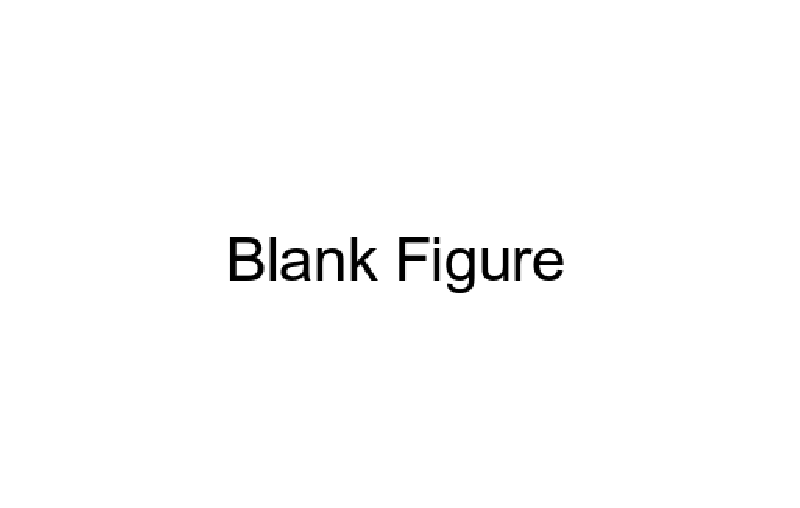
\includegraphics[width = 0.5\columnwidth]{tex/2-neutrinos-images/blank.eps}
%\caption{Figure in a subfolder.} 
%\label{fig:test2}
%\end{figure}

